\chapter{Background}
\label{cha:background}
We use existing cloud-based solutions as building blocks for the development and deployment of our solutions, which we present in more detail in this chapter. We focus on technical details relevant to our system and general information such as pricing and other important characteristics. Section~\ref{sec:in_memory} presents general principles of in-memory data management and an introduction to Redis~\cite{noauthor_redis_nodate-3}, one of the most popular open-source in-memory databases. Section~\ref{sec:aws_services} provides an overview of several AWS services that are relevant in the context of our work.

\section{In-Memory Data Management}
\label{sec:in_memory}
% Both relational and NoSQL databases are in-memory databases that provides different mechanism for data storage and retrieval~\cite{zhang_-memory_2015}.
In-memory data processing is becoming increasingly popular in numerous application areas. The ability to manage and process data at high speed enables not only big data systems to support interactive data analytics but also provides new opportunities for servers to use in-memory data management as a distributed cache for frequent data storage and retrieval~\cite{zhang_-memory_2015}. The higher throughput and lower latency of memory enable much faster processing compared to hard disks~\cite{chen_towards_2016}. This, combined with the fact that the price of memory is dropping by a factor of ten every five years, while capacity and bandwidth continue to increase, and it is not surprising that in-memory data management is a popular field in academia and industry~\cite{zhang_-memory_2015}. 

~\\
There are two main types of modern database systems: relational (SQL) and non-relational (NoSQL) databases. Relational databases have a table-based data structure with a predefined schema, while non-relational databases do not use a predefined schema and store unstructured data. Non-relational databases can be based on key-value pairs, documents, column-oriented, or graphs. Besides the different structures for storing data, the main difference is the implicit properties. Normalization in relational databases reduces storage requirements by reducing data duplication and contributes to data integrity. This is also an important point for the performance of relational and non-relational databases, but direct comparison is always tricky because it depends very much on the context. In principle, relational databases can satisfy the transactional properties of ACID\footnote{A set of properties for database transactions: Atomicity, consistency, isolation, durability.}~\cite{garcia-molina_database_2008}, while non-relational databases as distributed systems are coupled to the CAP theorem\footnote{The CAP theorem states that a distributed system can only achieve two of the three properties: Consistency, Availability and Partition Tolerance.}~\cite{sadalage_nosql_2012}. Another important point is the scaling of the systems. While relational databases are usually scaled vertically, non-relational databases can be scaled more cost-effectively by scaling horizontally. 

\subsection{NoSQL}
\label{subsec:nosql}
Coming back to in-memory data management, it is important to know that there are relational and non-relational in-memory databases. NoSQL databases are often motivated by their simplicity, favoring availability compared to consistency, and the ability to scale horizontally by adding more servers, which makes them perfect for building a distributed cache~\cite{zhang_-memory_2015, mohamed_relational_2014}. For the purpose of this work, we focus on non-relational data storage systems, which are divided into four categories~\cite{mathew_analysis_2015}:
\begin{itemize}
  \item \textbf{Key-Value Stores.} The simplest type of NoSQL databases are key-value stores, where data is stored in unstructured form. Key-value stores are highly partitionable and therefore allow perfect horizontal scaling. 
  \item \textbf{Document Stores.} Document databases extend simple key-value storage by storing the value in a structured format, a document. Since the value is stored in a more structured form, indexing by specific fields is possible and not limited to simple queries by key, as with key-value stores.
  \item \textbf{Column-Oriented Stores.} Similar to relational databases, column-oriented databases are table-based, but they store the data in columns instead of rows. While relational databases query the table row by row, column-oriented stores allow for faster querying when only a few columns are of interest.
  \item \textbf{Graph Databases.} Compared to relational databases, where data is used to express relationships, graph databases store relationships directly as edges and focus heavily on the connection between data nodes.
\end{itemize}

% In-Memory Data processing using Redis Database~\cite{kaur_-memory_2018}.
% In-Memory Big Data Management and Processing: A Survey~\cite{zhang_-memory_2015}.
% Relational vs. NoSQL Databases: A Survey~\cite{mohamed_relational_2014}.

\subsection{Redis}
\label{subsec:redis}
Redis is one of the most popular, open-source, in-memory non-relational databases in the category of key-value stores~\cite{noauthor_redis_nodate-3}. Redis achieves high performance compared to other key-value databases and relational databases while providing a simple, domain-independent \code{get/set} API~\cite{puangsaijai_comparative_2017, adya_fast_2019}. By supporting data structures other than strings (e.g., lists, sets, and hashes), Redis is not a typical key-value store such as Memcached. It also supports more advanced features, but these are not relevant in the context of this work. The book \emph{Redis in Action}~\cite{noauthor_redis_nodate} gives a good overview of what Redis can do and which problems can be solved with Redis. Redis provides a fully functional in-memory remote database, yet it is often used as a caching service for a primary database to improve performance. Amazon provides two managed services for Redis: Amazon MemoryDB for Redis~\cite{noauthor_amazon_nodate-3} and Amazon ElastiCache for Redis~\cite{noauthor_amazon_nodate-1} which is described in more detail in Section~\ref{subsec:elasticache}. Both services provide a fully managed in-memory database service billed by instance hours per node. However, ElastiCache is designed to accelerate the performance of a primary persistence database, while MemoryDB is designed to be used as the primary database~\cite{noauthor_introducing_2021}.

\paragraph{Persistence.} While Redis is designed to handle high rates of read requests and generally provide high availability, failover must always be considered. Redis provides two forms of persistence in the event of a failure by writing the in-memory data to disk. The first method dumps the data when a specified condition is met, or Redis receives the specified command. In contrast, the second method is similar to a write-ahead log that maintains persistence by writing operations to disk. To ensure high availability, a particular mode of the Redis server can be used for automatic failover management from a master to one of its replicas, called \emph{Redis Sentinel}.  

\paragraph{Scaling.} Redis supports replication in the form of a master/replica design. The master instance is responsible for processing writes, while multiple read replicas can scale for higher rates of read queries. The read replicas receive a copy of the entire database and the respective updates of the writes performed on the master instance. The well-known sharding method can be used to increase the total available memory but is also used to increase write throughput. This allows Redis to split the data across multiple machines, resulting in multiple master instances when the limit of a single machine is reached, resulting in a Redis Cluster. Interestingly, Redis handles reads/writes with a single-thread design, avoiding the overhead of synchronizing with locks, while most of the time, either the network or memory is the bottleneck. If the server contains multiple CPUs, one could also start multiple instances on the same server and treat them as different servers instead of using multiple machines if the CPU is the bottleneck.

\paragraph{History.} We mentioned Redis Sentinel for automatic failover above. It is worth noting that Redis did not initially support sharding or automatic failover. Before creating a distributed system with sharding support, Redis Sentinel was developed to provide automatic failover management for the master/replica topology. Later, the Redis Cluster project was developed to distribute data to different machines using sharding and multiple master instances while providing automatic failover management. As of Redis 3.0, both techniques are integrated into Redis~\cite{silva_redis_2015}.

\paragraph{Revisiting the CAP Theorem.} The CAP theorem states that a distributed system cannot provide consistency, availability, and partition tolerance at the same time. Strictly speaking, Redis is neither consistent nor available under network partitions~\cite{silva_redis_2015}. However, Redis attempts to provide the best possible guarantees with respect to both but focuses on building a fast in-memory system. For this reason, Redis is often used as a caching layer for read-intensive workloads, while the system is backed by another primary database that provides strict guarantees. The book \emph{Redis Essentials}~\cite{silva_redis_2015} provides more information on this topic and the capabilities of Redis Sentinel and Redis Cluster.

\paragraph{Redis as a Cache.} In Redis, data can be explicitly removed with \code{del} operations. However, another way to manage the data is to specify time to live, and Redis will automatically remove the key when it expires. There is also the possibility to declare an eviction policy so that once the memory limit is reached, Redis uses the policy to manage the data. Examples are \emph{noeviction}, which results in an error when the limit is reached, LRU approach where the least recently used key is removed, and some more. Some hybrid policies combine a traditional eviction policy with the specified TTL. So while Redis provides a fully functional in-memory remote database, the design clearly targets the use case of Redis as a caching layer.


% Towards Scalable and Reliable In-Memory Storage System: A Case Study with Redis~\cite{chen_towards_2016}.
% A Comparative Study of Relational Database and Key-Value Database for Big Data Applications~\cite{puangsaijai_comparative_2017}.
% Workload Analysis of a Large-Scale Key-Value Store~\cite{atikoglu_workload_2012}.
% Redis in Action~\cite{noauthor_redis_nodate}.
% Redis Essentials~\cite{silva_redis_2015}.
% Multi-thread performance on a single thread in-memory database~\cite{lubis_multi-thread_2015}.


\section{AWS Services}
\label{sec:aws_services}
The following section describes some of the more than 200 available services offered by Amazon Web Services (AWS)~\cite{noauthor_cloud_nodate}. Since we either use the services as a building block in our system or refer to them in the discussion, we will briefly introduce the services with information relevant to this work. All prices in this section refer to the Europe(Frankfurt) region and correspond to the information on the official website for the respective service.


\subsection{Simple Storage Service (S3)}
\label{subsec:s3}
Amazon Simple Storage Service (S3) focuses on a simple design to provide users with robust and simple object storage~\cite{noauthor_cloud_nodate-1}. There is no specific storage hierarchy other than buckets, but with some naming convention for the keys of the objects, the user can enforce a folder structure supported by the S3 console. However, the actual data model is a flat structure of buckets and the objects stored in each bucket. An object in the context of S3 is the value stored as an unstructured sequence of bytes and some metadata. S3 provides a simple key-value store that allows you to store an unlimited number of objects in buckets, with an object size limit of 5 TB. The bucket name, key, and version ID uniquely identify an object, while the authentication process ensures access control. Depending on the use case and requirements, S3 supports different storage classes: Standard, Reduced Redundancy Storage (RRS), and GLACIER~\cite{noauthor_amazon_nodate-2}. We focus on the standard class in this work.

\paragraph{Pricing.} The total cost of S3 is made up of several components, centered around the approach that users pay only for what they use, which is more or less unusual for storage services. So the cost are based on some key metrics: the required storage capacity, number of requests, and the amount of data transferred. For storage capacity, Amazon offers different price tiers, which lead to a cheaper price per GB above a certain amount. The price per GB is \$0.0245 for the first 50 TB/month. For requests, the price depends on the type of query and is given as the price per 1000 queries, for \code{PUT, COPY, POST, LIST} \$0.0054 is charged, while \code{GET, SELECT} and all other queries cost \$0.00043.

\subsection{Elastic Compute Cloud (EC2)}
\label{subsec:ec2}
Amazon Elastic Compute Cloud (EC2) is one of the most well-known of Amazon Web Services~\cite{noauthor_secure_nodate}. The service provides users with scalable computing capacities with configurable security, networking, and storage capabilities. The unique virtual computing environments are called instances and can be created and managed by the user through the EC2 console, the AWS CLI, or language-specific SDKs. Figure~\ref{fig:ec2_lifecycle} shows the lifecycle of an EC2 instance, which depends on whether the instance is deployed with an Elastic Block Store (EBS)\footnote{EBS allows block storage to be added to EC2 units in the form of SSD or HDD.} volume attached. This is the case in our deployment, and therefore the only states relevant for us are pending, running, stopping, and stopped. The Amazon Machine Image (AMI) is specified when an instance is created and used to boot the instance. Starting the instance is possible only when it is in the stopped state, while we can stop it when it is in the pending or running state. EC2 offers a wide range of instance types with different CPU, memory, storage, and network capacities combinations. We focus on the \code{t2.micro} instance with 1 vCPU (thread of the actual core), 1 GiB memory, and low to moderate network performance.

\begin{figure}[ht!]
  \begin{center}
      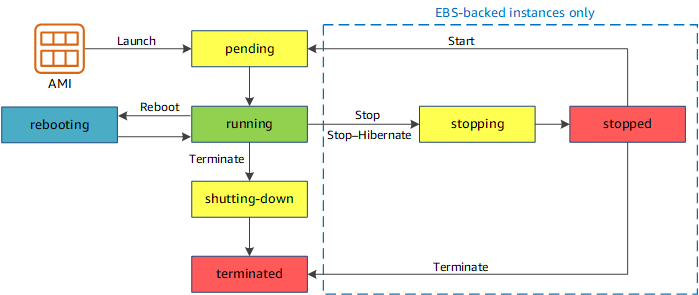
\includegraphics[width=0.8\textwidth]{figures/ec2_instance_lifecycle.png}
      \caption{Illustration of the state transitions of an EC2 instance~\cite{noauthor_instance_nodate}.}
      \label{fig:ec2_lifecycle}
  \end{center}
\end{figure}

\paragraph{Networking.} The instance is given a private and a public IPv4 address, where the private address is not reachable over the Internet but can be used for communication between endpoints within the same Virtual Private Cloud (VPC)\footnote{Amazon VPC builds a virtual network environment that users can control at will.}, while the public address is reachable over the Internet. The private IPv4 remains associated with the network interface during the lifecycle, while a public IPv4 is reassigned each time the instance transitions to the running state. Security groups\footnote{Security groups allow users to control traffic and act as a custom virtual firewall.} can be used to configure a virtual firewall and restrict incoming and outgoing traffic based on type, protocol, port, and source.

\paragraph{Pricing.} The lifecycle shown is important later when our orchestrator manages the EC2 instance, but the lifecycle also plays a crucial role in understanding the EC2 billing process. Once an instance enters the running state, it will be charged for every second it keeps running, with a minimum of one minute. The price depends heavily on the instance type, the price for the \code{t2.micro} instance is \$0.0134 per hour. There are several ways to pay for EC2 instances: On-Demand, Savings Plans, and Spot Instances. Everything covered in this section refers to on-demand instances as we have used them. Savings plans reduce the price in exchange for a consistent amount of usage commitment. In contrast, Spot instances allow one to request free EC2 capacity at reduced prices, suitable for stateless, fault-tolerant, or flexible applications~\cite{noauthor_secure_nodate}.

\subsubsection{Application in Practice: Self-Hosted Redis}
The EC2 computing platform can be used to host a wide range of applications. The platform also offers the option of setting up a self-hosted Redis cluster. We use the term ``self-hosted'', even though the servers are deployed in the cloud, to illustrate the difference from the fully managed Amazon ElastiCache for Redis service in the next section. Getting a self-hosted Redis server up and running is relatively easy, while the real work is to monitor, maintain and properly configure it to meet requirements. Redis can be downloaded to an EC2 instance and set up as a daemon that runs when the EC2 instance enters the running state. When setting up a Redis cluster on multiple machines with sharding and multiple read replicas, the process to get each node up and running is similar. For the system administrator, the more challenging part is setting up each node configuration correctly to get the desired cluster.

~\\
Once the self-hosted Redis server or cluster is correctly configured, the system administrator is still responsible for keeping the instance only running if the cache is actually needed to avoid unnecessary costs. The system administrator is also responsible for scaling and maintaining the whole system. This entire process can be done manually or through automation. Later, we use the term ``automation process'' to describe the effort required for the system administrator to maintain and manage the self-hosted Redis server or cluster in a cost-effective manner using automation scripts. 

% Once the self-hosted Redis server or cluster is up and running, the system administrator is still responsible for scaling and maintaining the system. This entire process can be done manually or through automation. Automation requires querying the system for certain metrics and triggering scaling based on the metrics received. While there are some third-party tools available to assist the system administrator, it is still a significant amount of work to get everything up and running as intended.

% ElastiCache or Self-Hosted Redis on EC2: Which is the One For You?~\cite{noauthor_elasticache_nodate}.

\subsection{ElastiCache}
\label{subsec:elasticache}
Amazon ElastiCache is a Cache-as-a-Service on the AWS platform that uses either Redis or Memcached as its caching engine~\cite{noauthor_amazon_nodate-1}. The caching layer provided by ElastiCache is the same as self-hosted Redis, except that it is a fully managed service that takes care of provisioning, monitoring, and updating. More specifically, ElastiCache allows setting up Redis in a few clicks without ever touching the actual server(s). When creating an ElastiCache Cluster, one can enable or disable cluster mode and specify the number of replicas. If cluster mode is enabled, the number of shards can be specified, and the number of replicas is then considered the number per shard. The actual memory capacity is selected per node by specifying the desired node type, similar to the instance types for EC2. A few AWS-specific settings remain, but at this point, one is ready to confirm the creation of the ElastiCache cluster. Once up and running, the Redis cluster is configured, running, and seamlessly maintained without worrying about it. \emph{Performance at Scale with Amazon ElastiCache}~\cite{noauthor_performance_nodate} provides a good overview as well as the official documentation~\cite{noauthor_comparing_nodate}.

\paragraph{Cluster Mode Disabled vs. Enabled.}
% cluster mode enables vs disabled
Deploying a Redis cluster in disabled cluster mode is similar to Redis Sentinel, where the cluster is built from a single shard. Therefore, the only way to scale for more memory and better write throughput is to scale the node type. For read scaling, one can have up to five read replica nodes. In enabled cluster mode, vertical scaling is still possible, but sharding allows to scale the number of shards in addition to the number of replicas per shard. ElastiCache allows users to scale the node type or cluster configuration with a few clicks or through the AWS command-line interface without worrying about the underlying process of provisioning new instances or copying the data to the new node type.

\paragraph{Auto Scaling.}
% only available for cluster mode enabled
% https://docs.aws.amazon.com/AmazonElastiCache/latest/red-ug/Replication.Redis-RedisCluster.html
In August 2021, Amazon added a new feature to ElastiCache, Auto Scaling. Using AWS Application Auto Scaling and CloudWatch metrics, ElastiCache provides the ability to set automatic scaling policies. ElastiCache for Redis then automatically scales according to the policies by either adding/removing shards to the cluster or adding/removing read replicas, similar to the manual scaling described above. ElastiCache auto-scaling enables two types of scaling policies:
\begin{itemize}
  \item Target tracking scaling policies adjust resources based on a target value for a specific metric (e.g., memory usage).
  \item Scheduled scaling policy: Create scheduled actions to scale at specific times to handle predictable load changes.
\end{itemize}
It is important to note that auto-scaling is only available for ElastiCache in enabled cluster mode and that there are additional restrictions on ElastiCache node types. Only instance type families \code{R5, R6g, M5, M6g} and instance sizes \code{Large, XLarge and 2XLarge} are supported.

~\\
Scaling is possible both online and offline; although performance is affected by the computationally intensive scaling operations when scaling online, the server continues to process requests during the scaling process. The scaling process takes time, as it may require copying the entire database to a new node or online resharding, which involves rebalancing the shards. Thus, ElastiCache Auto Scaling ensures that a scaling action is not triggered lightly by monitoring whether the target value exceeds the specified metric over an extended period of several minutes~\cite{noauthor_auto_nodate}.

\paragraph{Pricing.} Billing is similar to EC2; there are on-demand and reserved nodes, with a discount offered for long-term commitments. The price is tied to the instance type used and is billed hourly instead of seconds for EC2. Node type names include a cache before their name, while naming conventions are the same as EC2 instances. The price per hour for \code{cache.t2.micro} is \$0.019. A portion of the memory is used for system overhead for each node. So while the EC2 node type \code{t2.micro} provides 1 GiB of memory, the corresponding ElastiCache node type \code{cache.t2.micro} provides only 0.555 GiB of memory. For the next larger node type \code{t2.small} with 2 GiB of memory, the corresponding ElastiCache node type provides 1.55 GiB of memory.

% ElastiCache or Self-Hosted Redis on EC2: Which is the One For You?~\cite{noauthor_elasticache_nodate}.
% Performance at Scale with Amazon ElastiCache~\cite{noauthor_performance_nodate}.

\subsection{Serverless Computing}
\label{subsec:lambda}
In general, Cloud computing or Infrastructure-as-a-Service (IaaS) is widespread and popular in practice. The pay-as-you-go model and the ability to scale without investing in hardware allowed cloud providers to take over a large portion of IT organizations' annual software and IT infrastructure spending. This clearly shows how popular cloud-based services like EC2 are. If resources are used as efficiently as possible, there is little for users to complain about. However, the responsibility for scaling lies with users, often leading to over-provisioning to accommodate sudden increases~\cite{castro_rise_2019}. While cloud providers are trying to ameliorate this problem by providing additional services such as EC2 Auto Scaling to help users use resources as efficiently as possible, cloud providers have also released a new approach to this problem, called serverless computing. 

~\\
Serverless computing is a computing platform like EC2 where servers are hidden from developers and code is run on demand and charged for actual execution time. Serverless computing is often referred to as Function-as-a-Service (FaaS). It allows developers to focus on implementation rather than the actual provisioning, resource allocation, and auto-scaling that is now handled by the cloud provider~\cite{eismann_serverless_2021}. The stateless nature of serverless computing is a challenge for applications that rely on state sharing or require data exchange~\cite{jonas_cloud_2019, klimovic_pocket_nodate}. Popular use cases are currently tightly coupled to the provided features of serverless computing, i.e., mainly event-driven workloads that can leverage the ability to scale from zero to infinity~\cite{jonas_cloud_2019}. However, it is important to note that serverless computing has attracted the attention of industry and academia and is constantly evolving to overcome particular challenges, making it a potentially leading platform in the future. Much work is done in benchmarking or architecture analysis~\cite{wang_peeking_2018, scheuner_function-as--service_2020}. There are also attempts to improve or extend the current architecture based on their needs~\cite{shahrad_serverless_2020, wawrzoniak_boxer_2021, wang_galleon_2021}. Others seek to solve challenges in the current paradigm of serverless computing~\cite{moyer_punching_2021, klimovic_pocket_nodate}. Exploring the possibilities of the serverless computing paradigm is of general interest and has led to several interesting projects that include serverless computing as a building block~\cite{wang_infinicache_2020, mahgoub_sonic_2021, thomas_particle_2020, noauthor_granular_nodate}.

~\\
In our work, we focus on AWS Lambda, Amazon's serverless computing service~\cite{noauthor_serverless_nodate}. We explore the capabilities of the serverless platform to provide in-memory caching capabilities. When creating a AWS Lambda function, the platform packages the function code into a container that runs on the multi-tenant cluster of machines managed by AWS. The user only has to specify the function code and some parameters about the function (runtime, architecture, memory, timeout), while the CPU is allocated proportionally to the amount of memory. Invoking a function is event-based, AWS supports several possible events: HTTP requests via Amazon API Gateway\footnote{Fully managed service for APIs.}, object changes on S3, table updates in Amazon DynamoDB\footnote{Fully managed, key-value NoSQL database.}~\cite{noauthor_fast_nodate}, or simply via the Invoke API provided by their SDK. The Invoke API supports synchronous (wait for response) and asynchronous calls. 

\begin{figure}[ht!]
  \begin{center}
      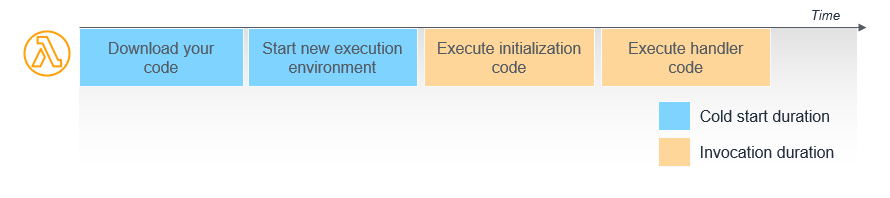
\includegraphics[width=0.8\textwidth]{figures/lambda_invoke.png}
      \caption{Illustrates the process of setting up an execution environment for AWS Lambda and then running the function code~\cite{noauthor_operating_2021}.}
      \label{fig:lambda_invoke}
  \end{center}
\end{figure}

\paragraph{Execution Environment.} Once the function is invoked, an execution environment on a Lambda Worker is created or assigned if a matching one already exists. Each execution environment may be used for only one concurrent invocation, while many instances of the same function can be executed concurrently. AWS Lambda continuously monitors and manages the execution environments, creating new environments and destroying old ones. Creating an execution environment includes downloading the code for the function and setting up the environment with the memory, runtime, and configuration as specified by the user. Once the environment setup is complete, Lambda executes the initialization code before executing the actual handler code, as shown in Figure~\ref{fig:lambda_invoke}. The first two steps are also referred to as a \emph{cold start}, which adds latency to the invocation process but is not charged for. After the function returns, Lambda keeps the execution environment for a non-deterministic period of time to optimize resource management and performance. Thus, if a new request for the same function arrives on time, the execution environment can be reused, resulting in a faster startup time, called a \emph{warm start}~\cite{noauthor_security_nodate, noauthor_operating_2021}.

\paragraph{Reusable Execution Environments.} The cold start concept compared to warm start has some additional effects despite the shortened start time. Reusing the execution environment also means that local state and even outgoing connections remain available. This can be used to save costs by reducing the actual execution time, as stated in the official documentation, but also provides many opportunities to use the serverless platform as a pay-as-you-go storage~\cite{wang_infinicache_2020}, which may not have been their intention. The duration that the execution environment remains is not deterministic, making it challenging to use this mechanism reliably. For security and data leakage reasons, care should be taken when using the execution environment to store data across invocations.

\paragraph{Networking.} Lambda function in a VPC does not have access to the Internet but can connect to other services in the same VPC. The significant problem is that AWS Lambda blocks inbound network connections but supports outbound TCP/UDP connections. NAT traversal techniques can be used to work around this limitation, for example, to allow direct communication between serverless functions~\cite{moyer_punching_2021}. 

\paragraph{Pricing.} Billing is based on the number of requests to the function and the function execution duration. The duration includes only the time when the actual function code (initialization code and handler code) was executed. Billing granularity is much finer on a millisecond basis compared to EC2. The price per millisecond depends on the amount of memory specified by the user. The minimum amount of memory is 128 MB and costs \$0.0000000021 per 1ms, 1024 MB costs \$0.0000000167, while the maximum amount is 10240 MB for \$0.0000001667 per 1ms. The price per millisecond is linearly proportional to the amount of memory available and thus to the CPU capacity.
